%
%%%%%%%%%%%%%%%%%%%%%%%%%%%%%%%%%%%%%%%%%%%%%%%%%%%%%%%%%%%%%%%%%%%%%%%%%%%%%%%
% Fractio of gluon splitting in data
%%%%%%%%%%%%%%%%%%%%%%%%%%%%%%%%%%%%%%%%%%%%%%%%%%%%%%%%%%%%%%%%%%%%%%%%%%%%%%%
%
\chapter{Fraction of double $b$-hadron jets in data}\label{ch:gbbfraction}

%------------------------------------------------------------------------
\section{Maximum likelihood fits}\label{sec:LLFits}
%------------------------------------------------------------------------

Maximum likelihood (ML) information only parametrizes the shape of a 
distribution (i.e. one can determine fraction of signal events from 
MC fits but no number of signal events).

The extended version of the maximum likelihood approach adds an extra term
allowing the estimation of the absolute number of signal/background events.

%Adding pdfs
For N p.d.f.s, there are N-1 fraction coefficients that should sum to less 1. The remainder is by construction 1 minus the sum of all other coefficients.


Binned or unbinned MF fit. %Roofit presentation page 112

In most RooFit applications it doesn't matter. Internally binned data is represented the same way as unbinned data, a ROOT TTree with the bin coordinates.

Weights are supported in unbinned datasets. But use with care. Error analysis in ML fits to weighted unbinned data can be complicated...

\subsubsection{Unbinned fits}


\subsubsection{Fitting and likelihood minimization}

What happens when you do pdf->fitTo(*data)?

- Construct object representing -log of (extended) likelihood

- Minimize likelihood w.r.t floating parameters using {\sc MINUIT}. % [REFERENCIAS].




%------------------------------------------------------------------------
\section{Results}\label{sec:FitsResults}
%------------------------------------------------------------------------

True fractions predicted by {\sc Pythia} Monte Carlo generator in Fig.~\ref{fig:truefractions}


\begin{figure}[tp]
\centering
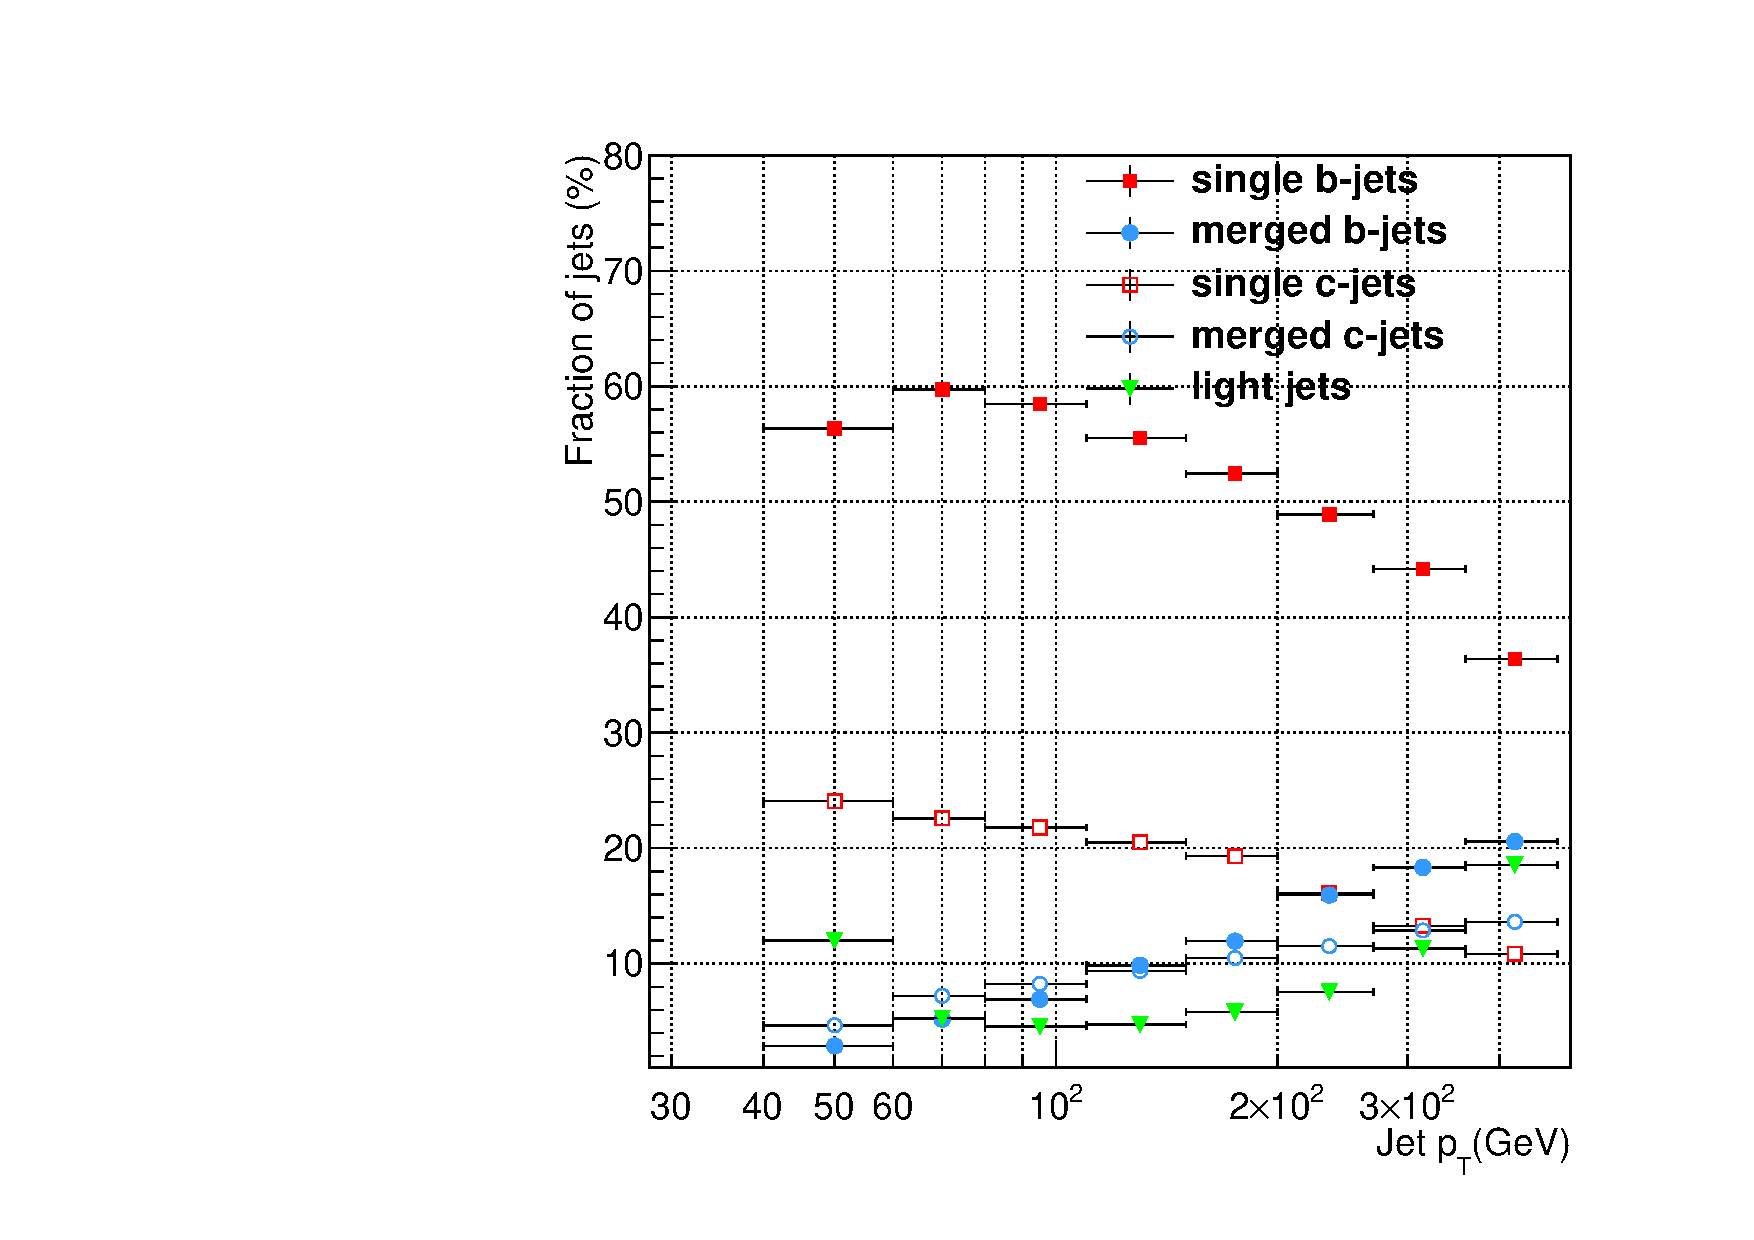
\includegraphics[width=0.9\textwidth]{TrueFractions_NominalPythia.pdf}
%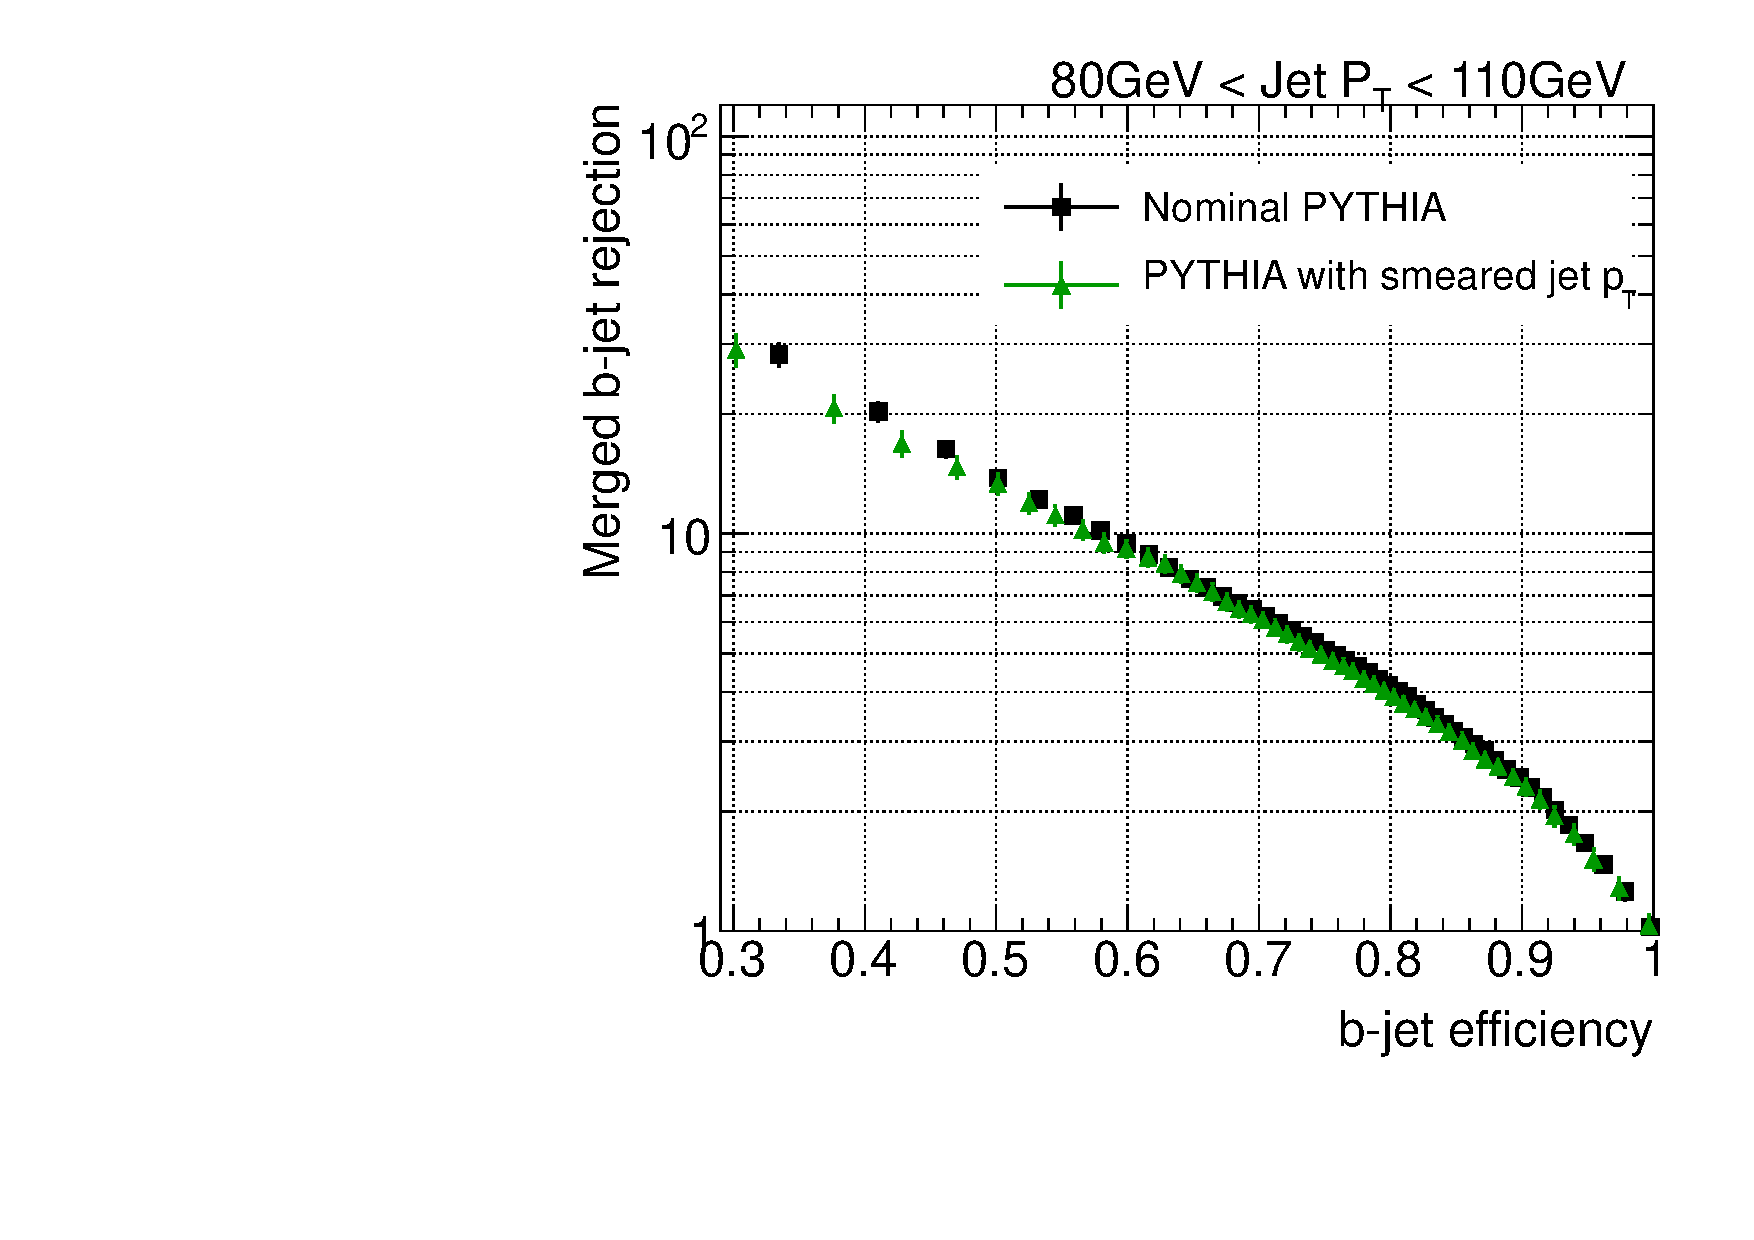
\includegraphics[width=0.49\textwidth]{FIGS/systematics/LlhoodKDE_ISO_SmearedJetPt_FIXEDBUGTest_rejvseff080.pdf}
\caption{Pythia predictions of the fractions of tagged single-b, merged-b, single-c, merged-c-jets and light jets in a Monte Carlo dijet sample.}
\label{fig:truefractions}
\end{figure}


5 and 3 free parameter fits were performed. Given that single-b (mereged-b) and single-c (merged-d) templates are hard to distinguish, we fixed single-c (merged-c) fractions to single-b (merged-b) ones.
%PARA JUSTIFICAR QUE HACEMOS LOS FITS CON 3 PARAMETROS PODEMOS MOSTRAR LOS HISTOS Y DECIR QUE LAS CORRELACIONES SON MUY GRANDES (PONER NUMEROS). EN ALGUN MOMENTO TENDRA QUE HABER UN C-TAGGER.  EN DIJET TENEMOS SINGLE-C'S, EN TTbar NO HAY C'S, SI HAY MERGED-C PERO ES ALGO QUE QUEREMOS REMOVER DE TODAS MANERAS.



The results of the 3-parameter fits for all bins of $\pt$ are shown in table~\ref{tb:fitfractions}.

The fit results are shown in Figures~\ref{fig:fittemplates1} and~\ref{fig:fittemplates2}.


\begin{figure}[tp]
\centering
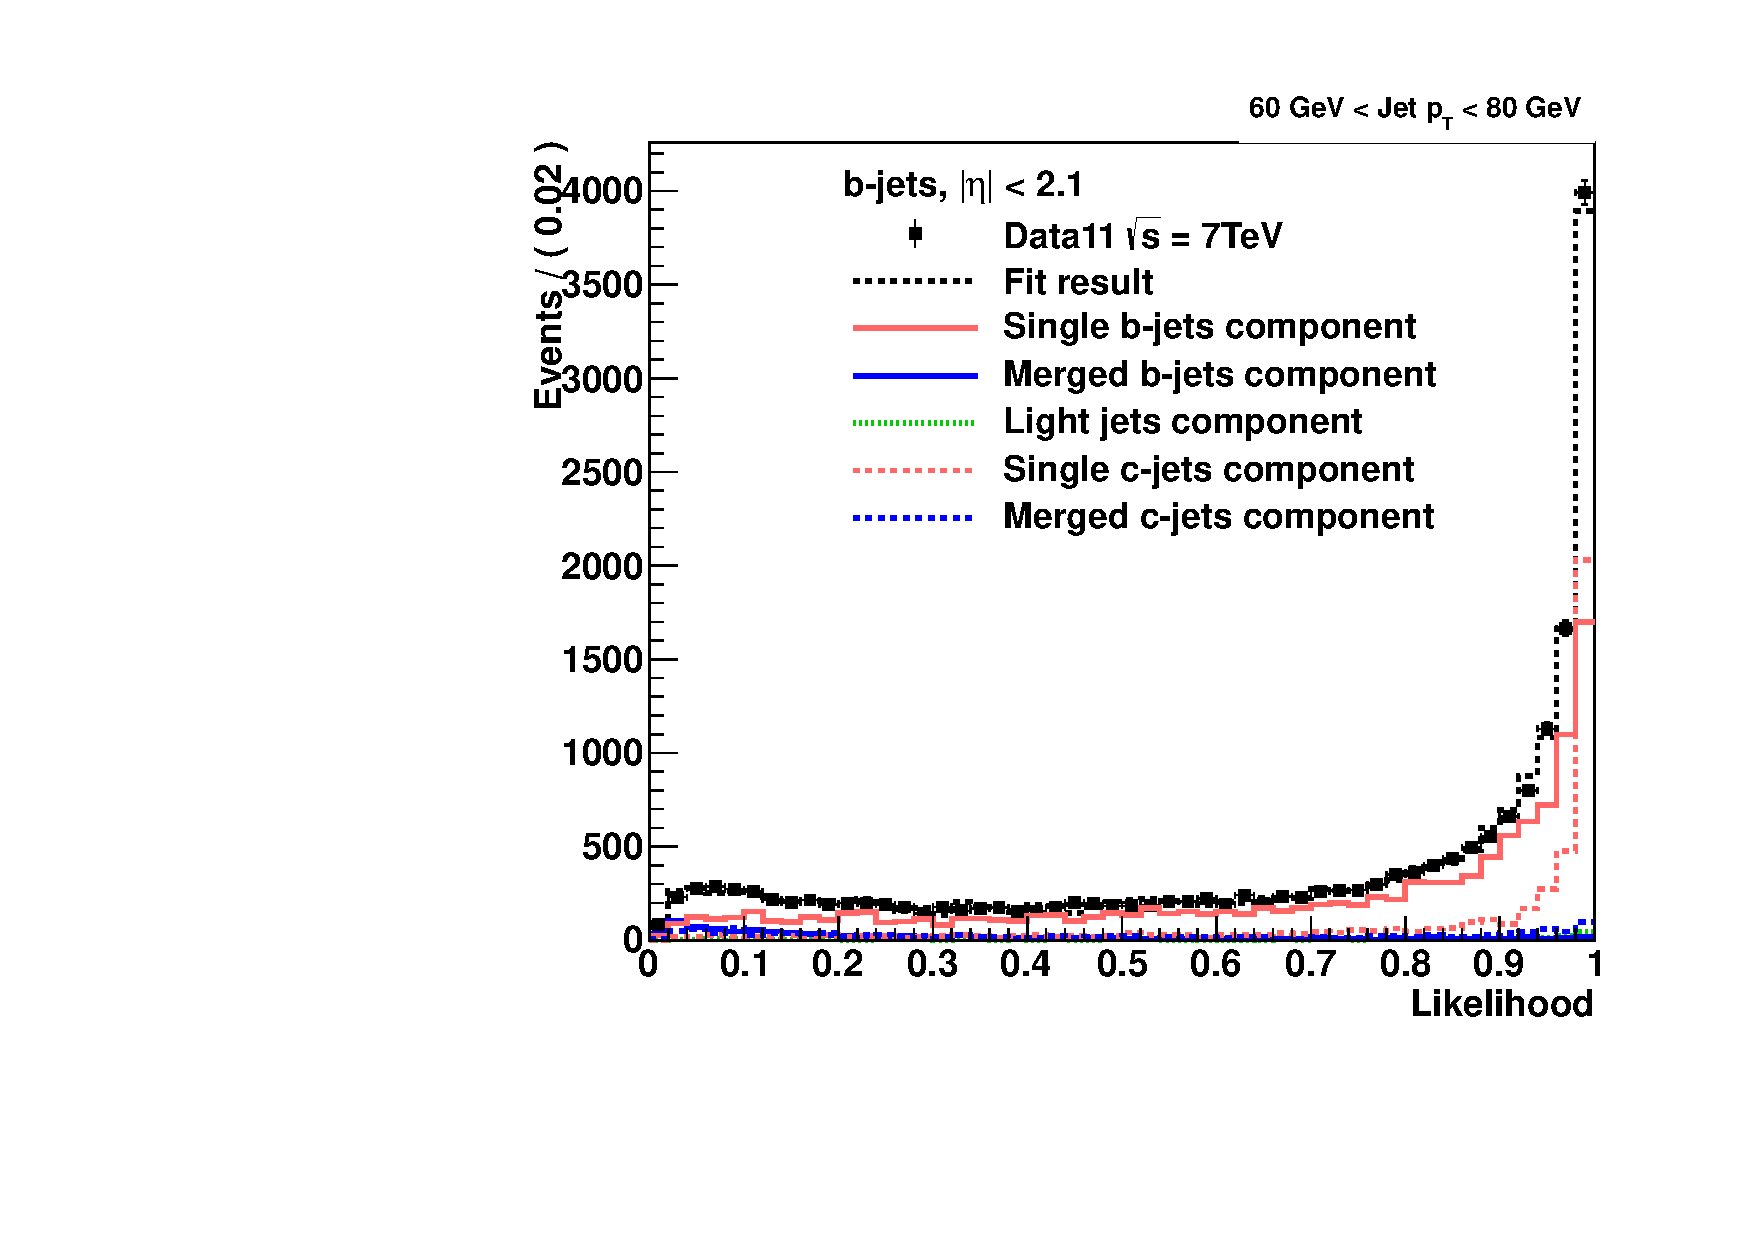
\includegraphics[width=0.7\textwidth]{FIGS/Fits/LikelihoodFit_3param_ETAFull_Bin1.pdf}
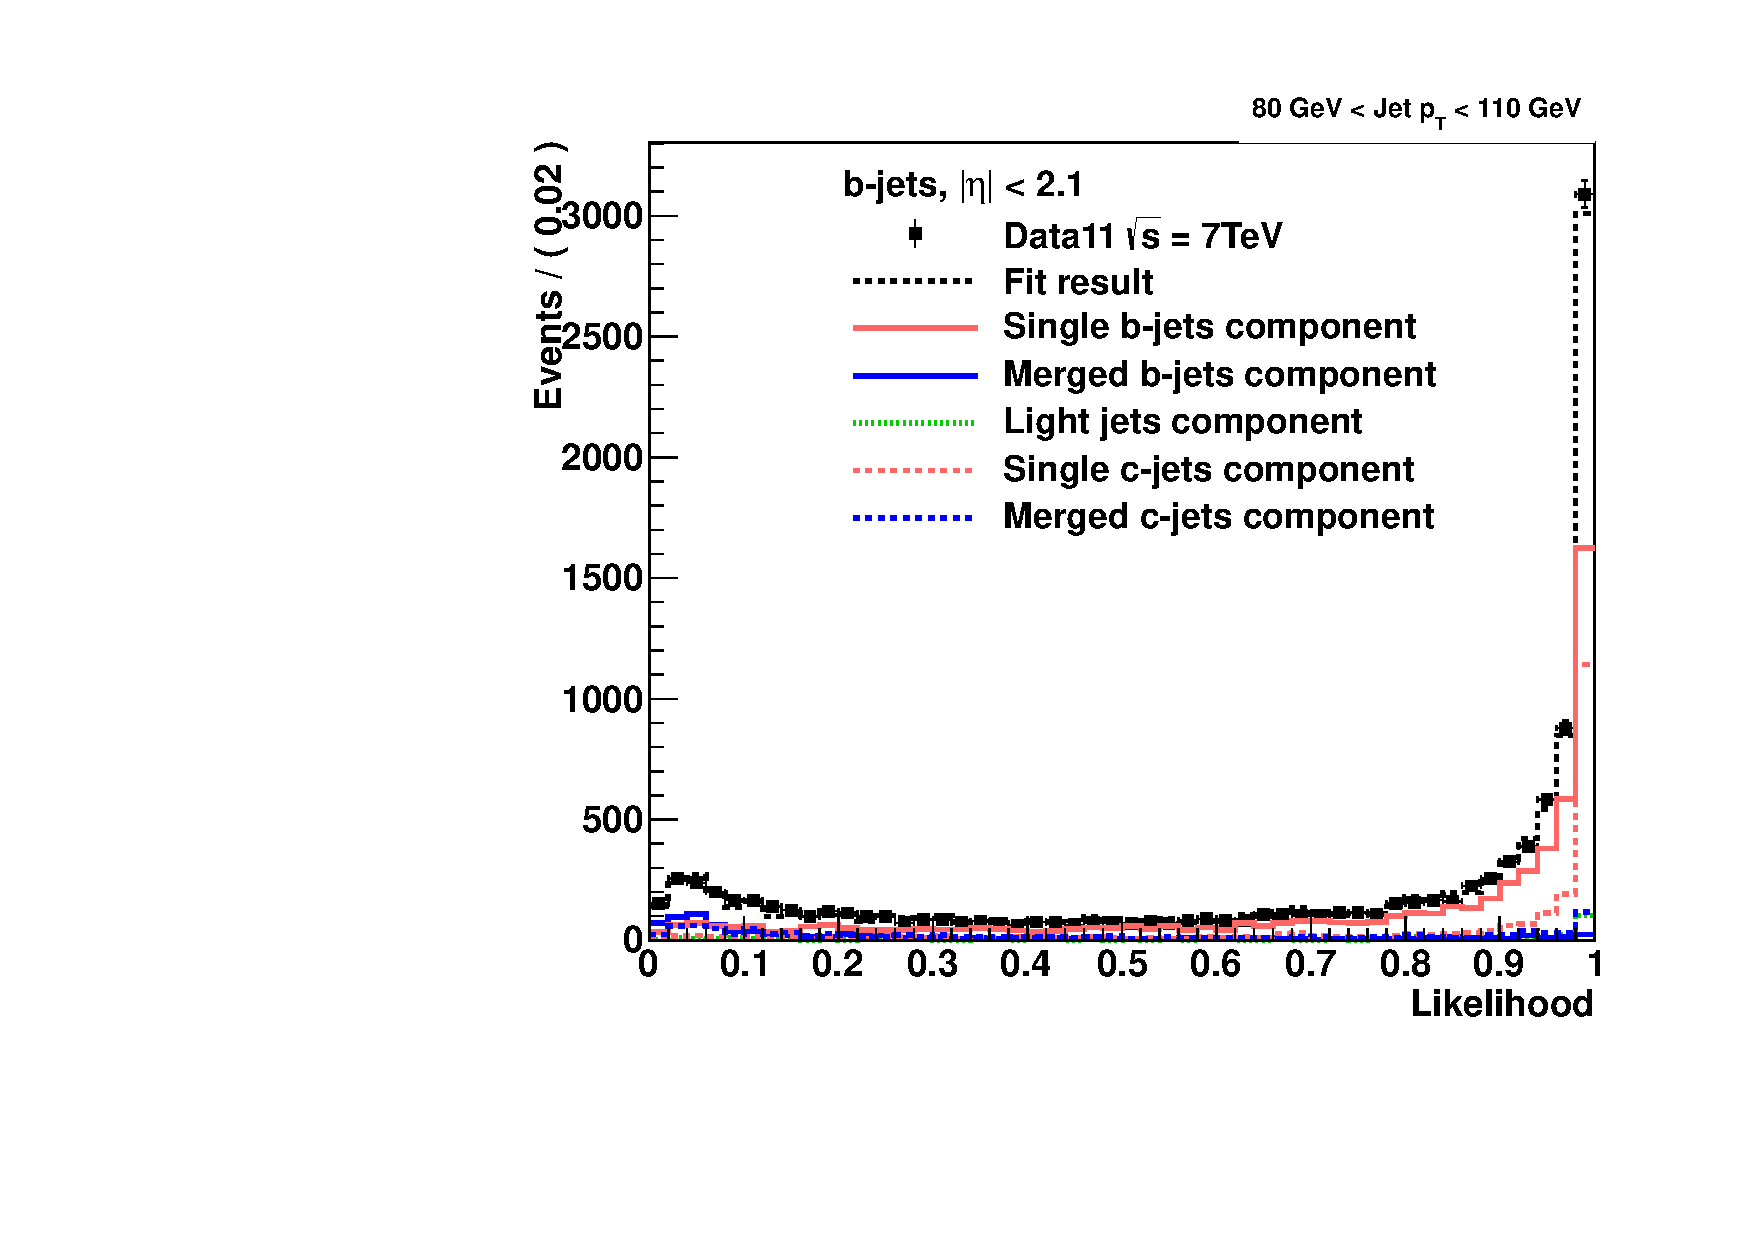
\includegraphics[width=0.7\textwidth]{FIGS/Fits/LikelihoodFit_3param_ETAFull_Bin2.pdf}
\caption{Monte Carlo templates for single, merged and light jets, fitted to data for jets between 60~GeV to 80~GeV and 80~GeV to 110~GeV.}
\label{fig:fittemplates1}
\end{figure}



\begin{figure}[tp]
\centering
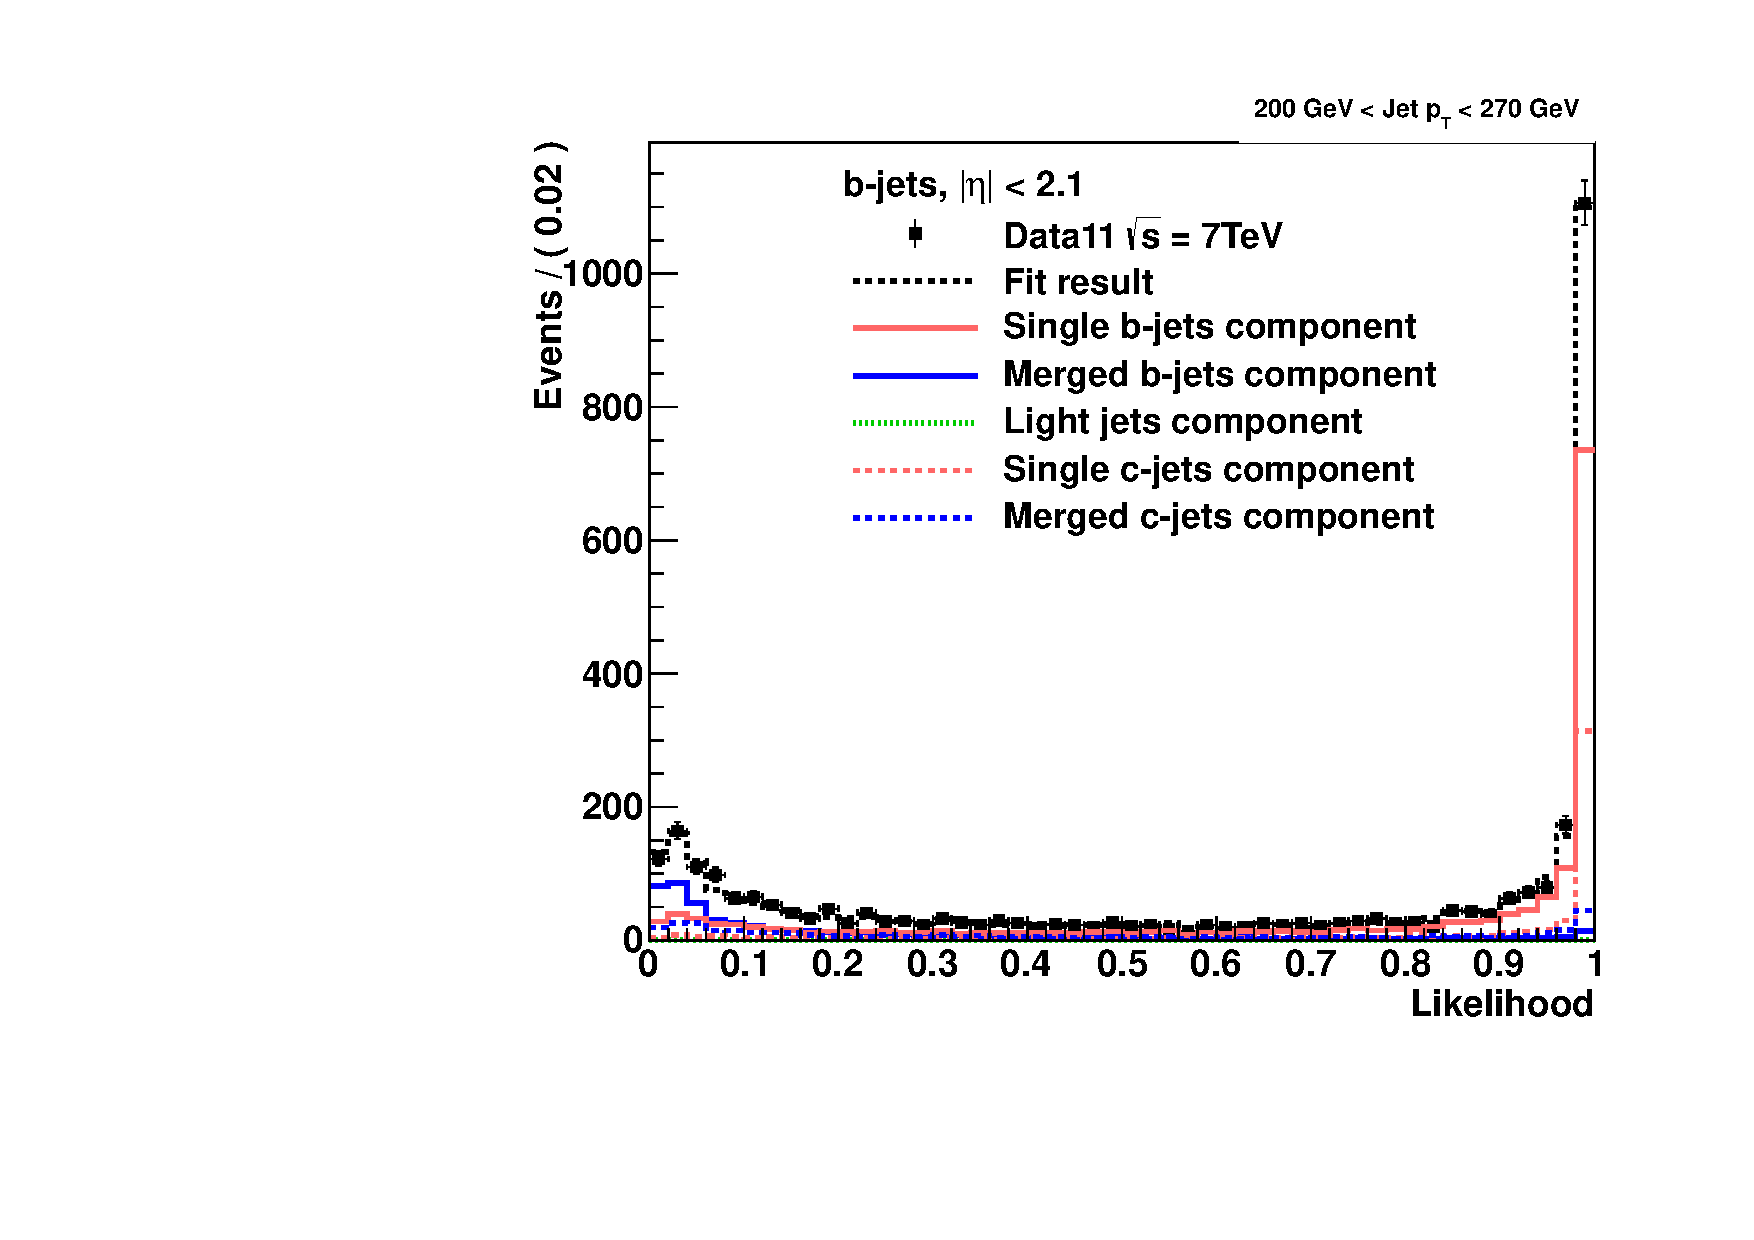
\includegraphics[width=0.7\textwidth]{FIGS/Fits/LikelihoodFit_3param_ETAFull_Bin5.pdf}
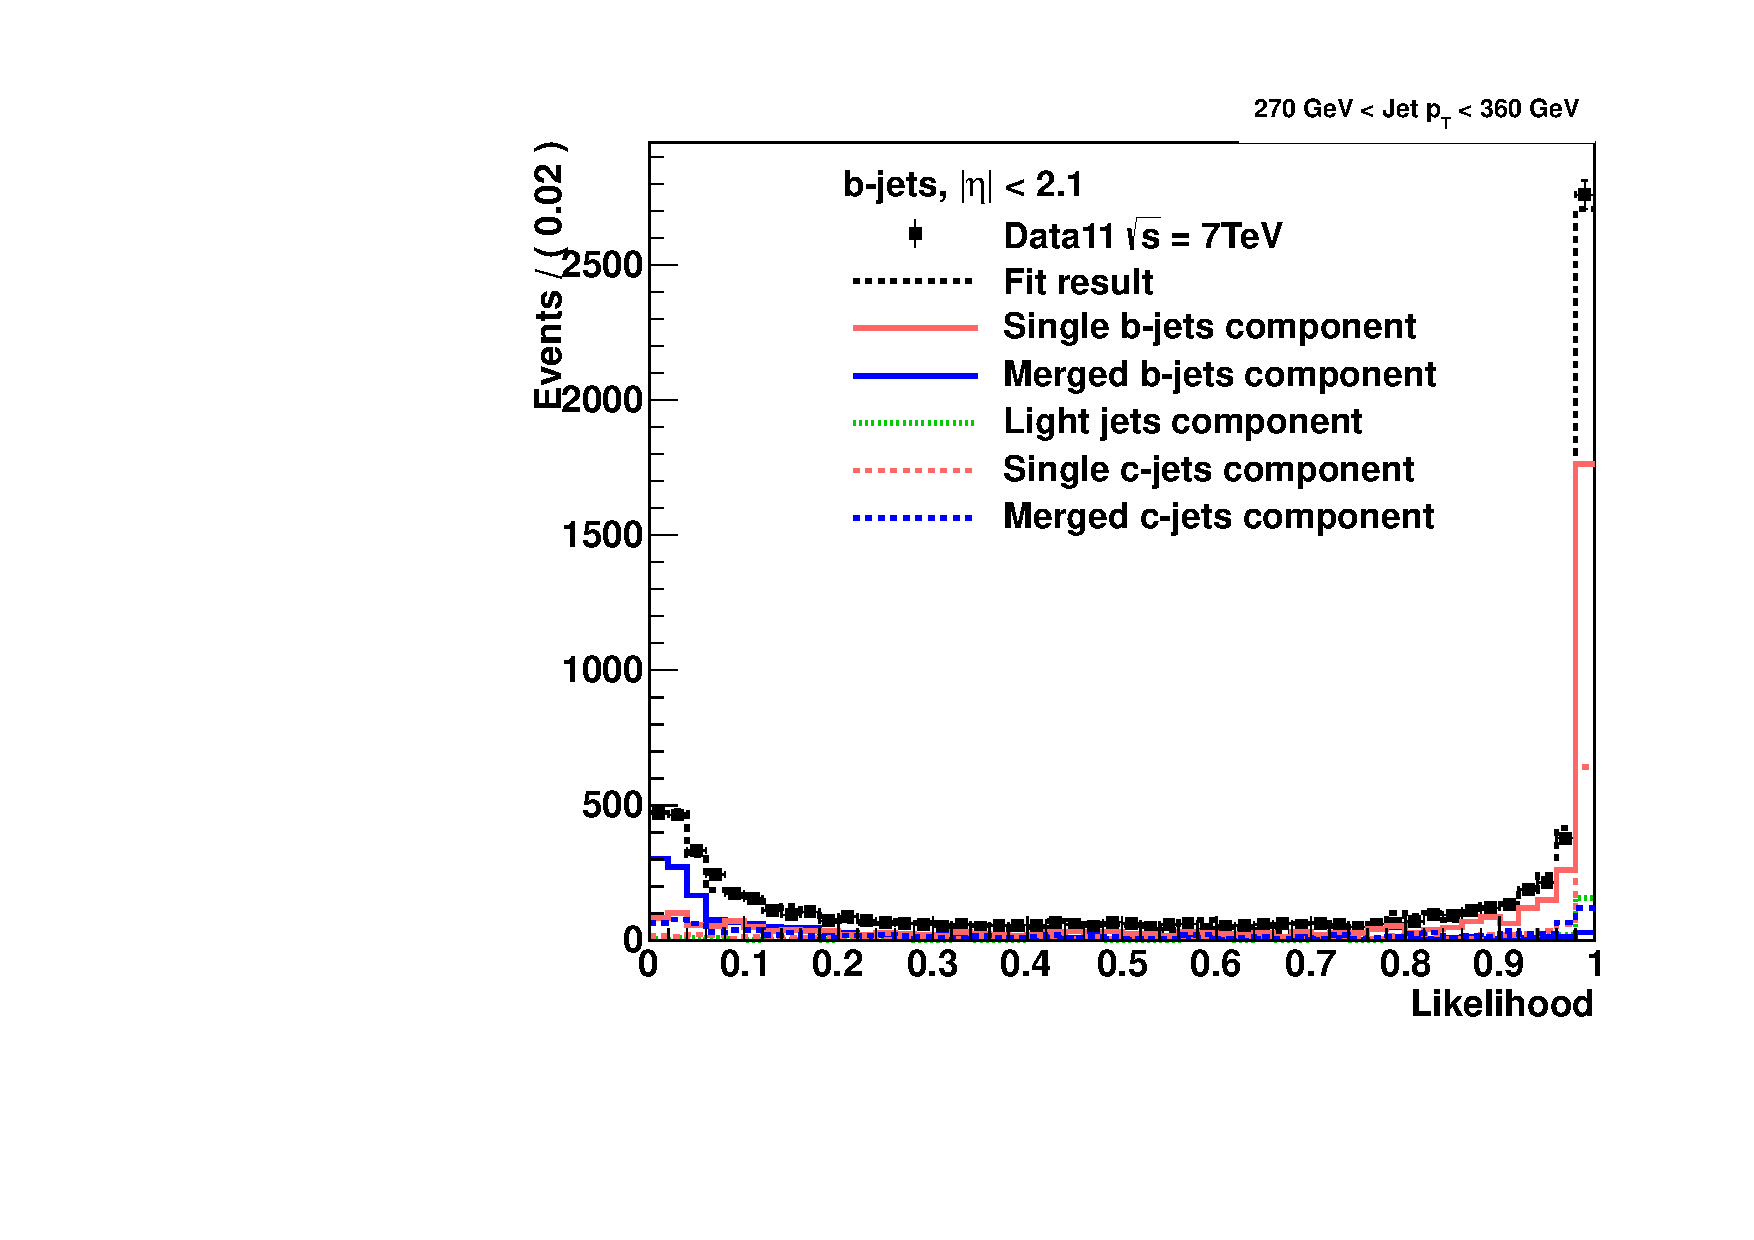
\includegraphics[width=0.7\textwidth]{FIGS/Fits/LikelihoodFit_3param_ETAFull_Bin6.pdf}
\caption{Monte Carlo templates for single, merged and light jets, fitted to data for jets between 200~GeV to 270~GeV and 270~GeV to 360~GeV.}
\label{fig:fittemplates2}
\end{figure}

\begin{table}[!hbt] %[h]
\renewcommand{\arraystretch}{1.2}
\centering
\begin{tabular}{ | c || c | c || c | c || c | c ||}
  \hline
  Jet $\pt$ & \multicolumn{2}{c||}{single $b$-jet} & \multicolumn{2}{c||}{merged $b$-jet} & \multicolumn{2}{c||}{~light jet~}\\ \cline{2-7}
    (GeV ) & fit result & ~stat.err. & fit result & ~stat.err. & fit result & ~stat.err.\\ \hline
   40 - 60 &  62\% &  3\%  &  ~~3\%  &  ~~1\% &  ~4\%  &  4\%   \\ 
   60 - 80 &  62\% &  1\%  &  5.2\%  &  0.4\% &  ~2\%  &  2\%   \\ 
   80 - 110&  57\% &  1\%  &  8.5\%  &  0.4\% &  ~3\%  &  2\%   \\ 
  110 - 150&  55\% &  2\%  &  ~13\%  &  ~~1\% &  ~1\%  &  4\%   \\ 
  150 - 200&  53\% &  3\%  &  ~15\%  &  ~~1\% &  ~0\%  &  4\%   \\ 
  200 - 270&  53\% &  5\%  &  ~17\%  &  ~~1\% &  -1\%  &  7\%   \\ 
  270 - 360&  48\% &  3\%  &  ~19\%  &  ~~1\% &  ~4\%  &  4\%   \\ 
  360 - 480&  39\% &  5\%  &  ~21\%  &  ~~1\% &  15\%  &  6\%   \\ \hline
\end{tabular}
\caption{Measured fractions of single, merged and light $b$-tagged jets in experimental data from 2011 run.}
\label{tb:fitfractions}
\end{table}







%------------------------------------------------------------------------
\section{Systematic uncertainties}\label{sec:FractionSystematics}
%------------------------------------------------------------------------

- TO DO: HACER JER SI PUEDO


In order to study the systematic uncertainties in the results the following contributions were evaluated:

\begin{itemize}\addtolength{\itemsep}{-0.4\baselineskip}
\item
uncertainty in the track reconstruction efficiency;
\item
uncertainty in the jet transverse momentum resolution;
\item
uncertainty in the jet energy scale.
%the effect of jet isolation
%\item
%other $\Delta R$ cuts for B-labeling and matching
\end{itemize}


\vspace{3mm}
The different contributions to the systematic uncertainty are summarized in Table~\ref{tb:systematicsfits}.
\begin{table}[!hbt] %[h]
\renewcommand{\arraystretch}{1.2}
\centering
\begin{tabular}{ | c | c |}
\hline
  ~~~~~~~Systematic source~~~~~~~ &~~Uncertainty~~\\ \hline
  track reconstruction efficiency  &    negligible\%        \\ 
  jet $\pt$ resolution  &    2\%        \\  
  jet energy scale  &    2\%        \\ \hline 
\end{tabular}
\caption{Systematic uncertainties.}
\label{tb:systematicsfits}
\end{table}



Changing the fractions merged-c/merged-b in 20\% only produced a marginal effect on the fit results. The total number of merged-c plus merged-b did not changed showing that in reality we are measuring the fraction of merged b+c together. The same result is expected if changing the single-c/single-b fraction.


%------------------------------------------------------------------------
\section{Enriched samples in single and merged $b$-jets}\label{sec:Enriched}
%------------------------------------------------------------------------

\subsubsection{Enriched sample in merged $b$-jets}



\subsubsection{Enriched sample in single $b$-jets}

The results of performing the fits on an data sample enriched in single $b$-jets is shown in tables~\ref{tb:fitfractions2btagS} to ~\ref{tb:fitfractions2btagL}. The model fitted to the data agrees well within statistics %THE TEMPLATES WORK WELL!
and the result is in agreement with the predictions made by {\sc Pythia} on a sample with the same level o of enrichment.  % (PODRIAMOS DECIR QUE LA FRACCION DE FLAVOR CREATION ESTA BIEN SIMULADA POR PYTHIA)


The fit results are shown in Figures~\ref{fig:fitenriched2btag1} and Figures~\ref{fig:fitenriched2btag2}.


\begin{figure}[tp]
\centering
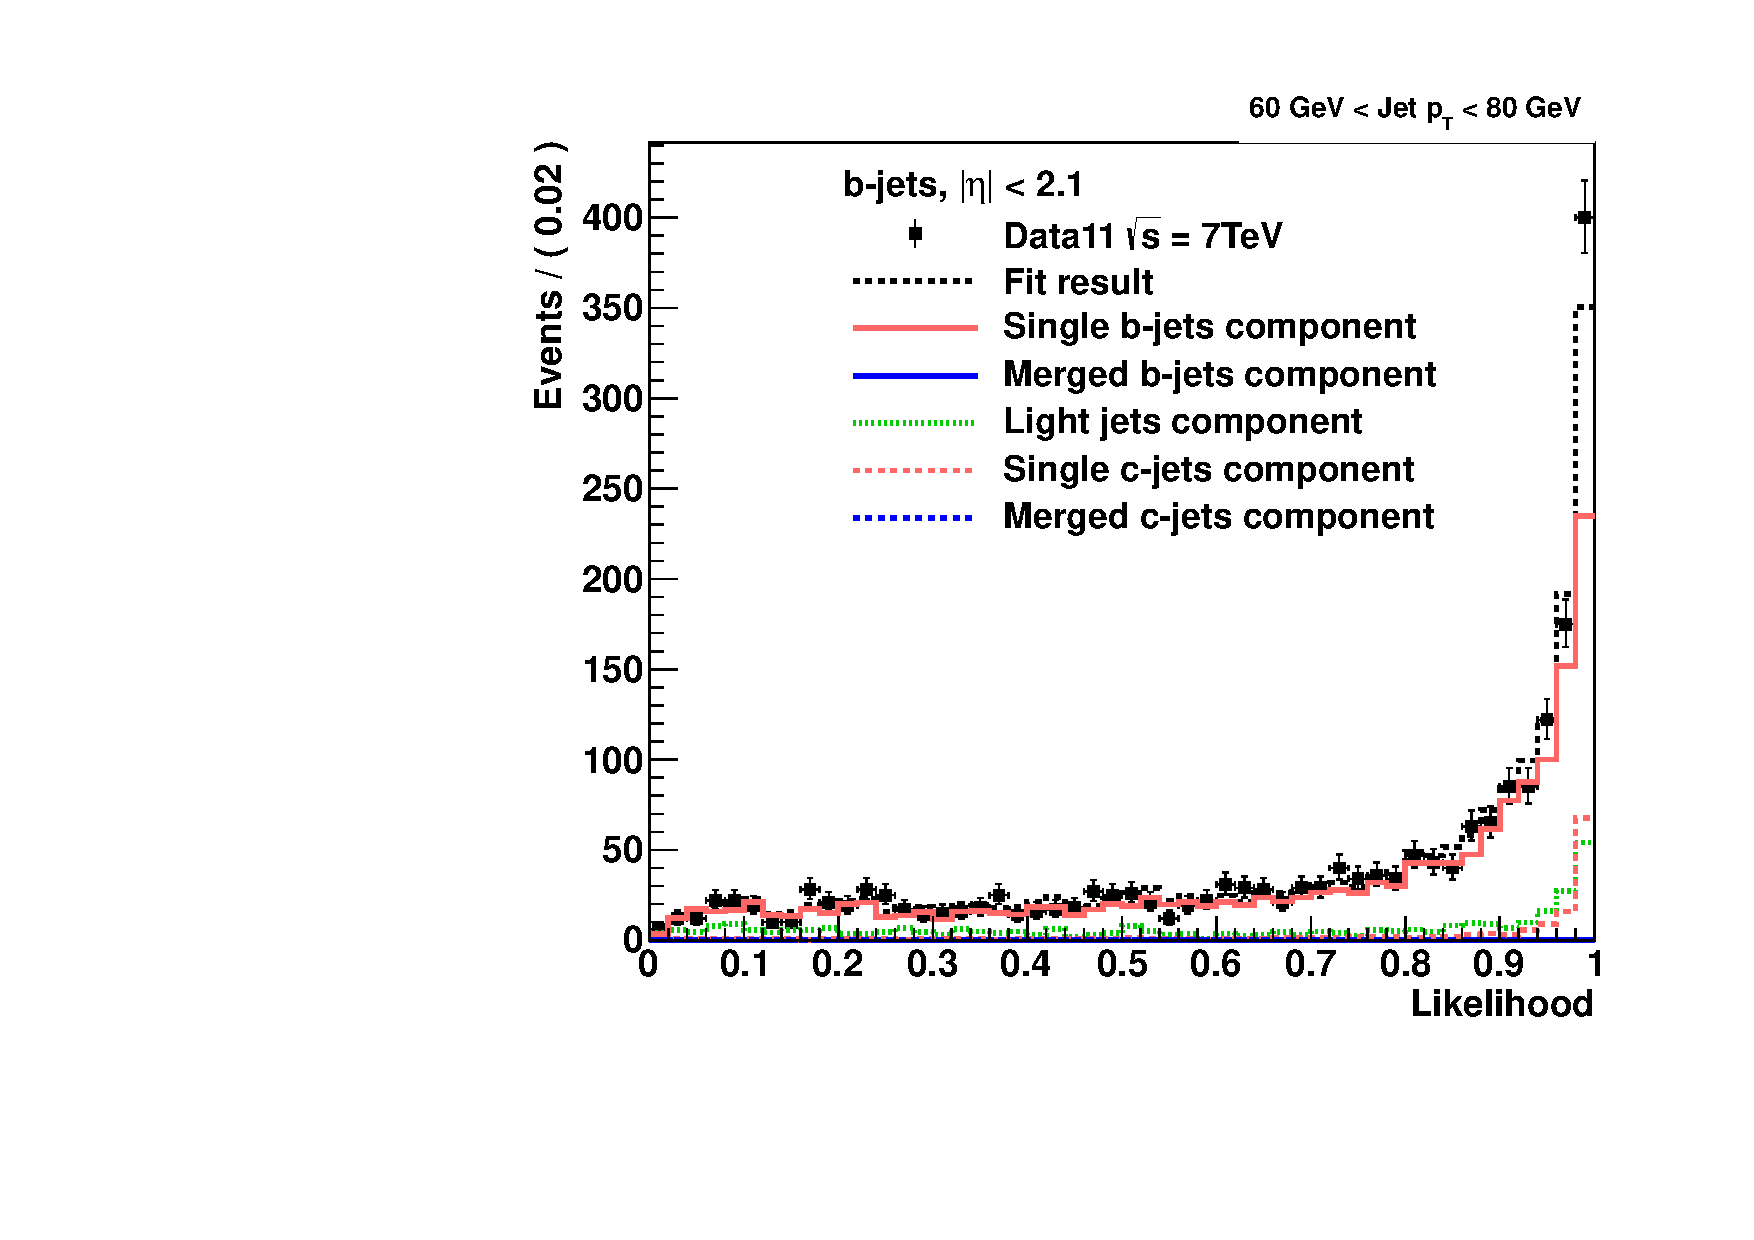
\includegraphics[width=0.7\textwidth]{FIGS/Fits/LikelihoodFit_3param_ETAFull_DataEnriched2btag_Bin1.pdf}
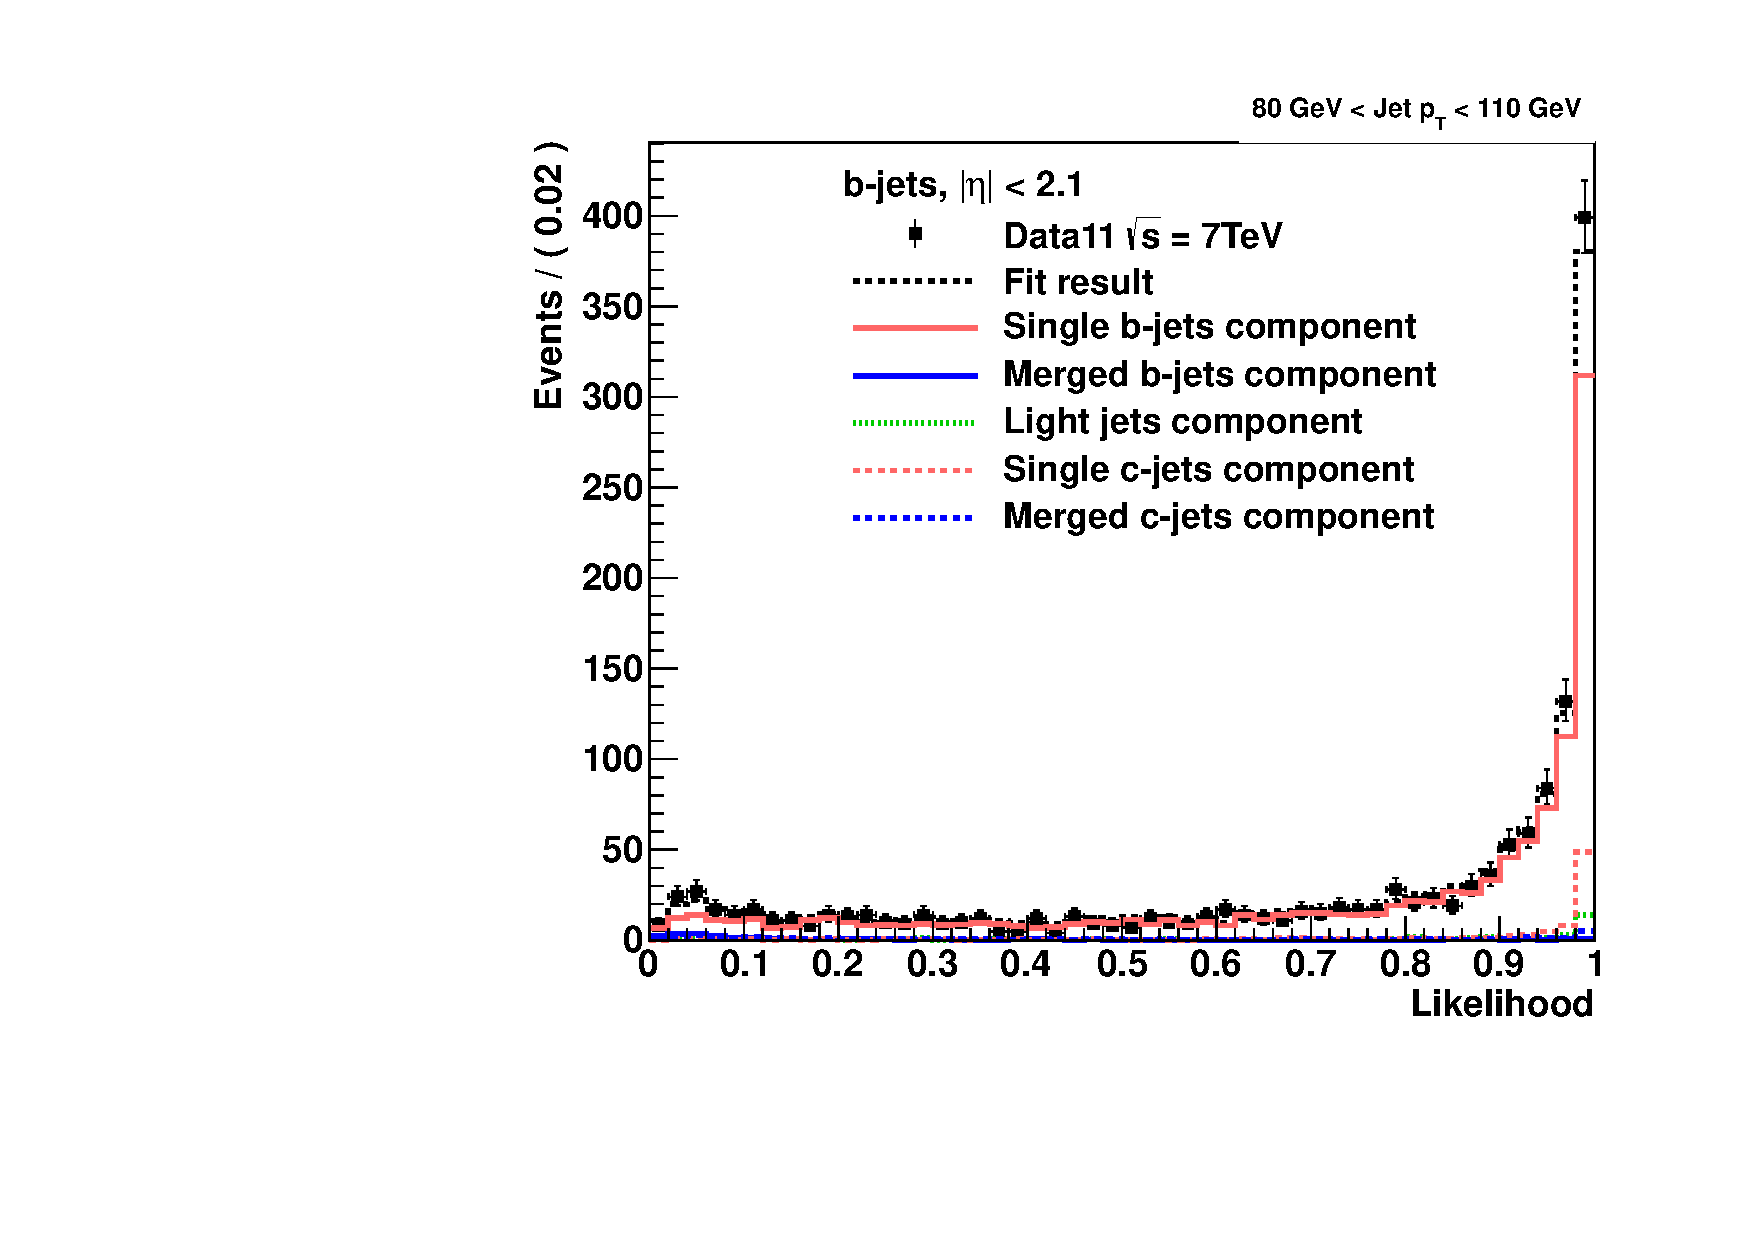
\includegraphics[width=0.7\textwidth]{FIGS/Fits/LikelihoodFit_3param_ETAFull_DataEnriched2btag_Bin2.pdf}
\caption{Monte Carlo templates for single, merged and light jets, fitted to data enriched in single $b$-jets, for jets between 60~GeV to 80~GeV and 80~GeV to 110~GeV.}
\label{fig:fitenriched2btag1}
\end{figure}



\begin{figure}[tp]
\centering
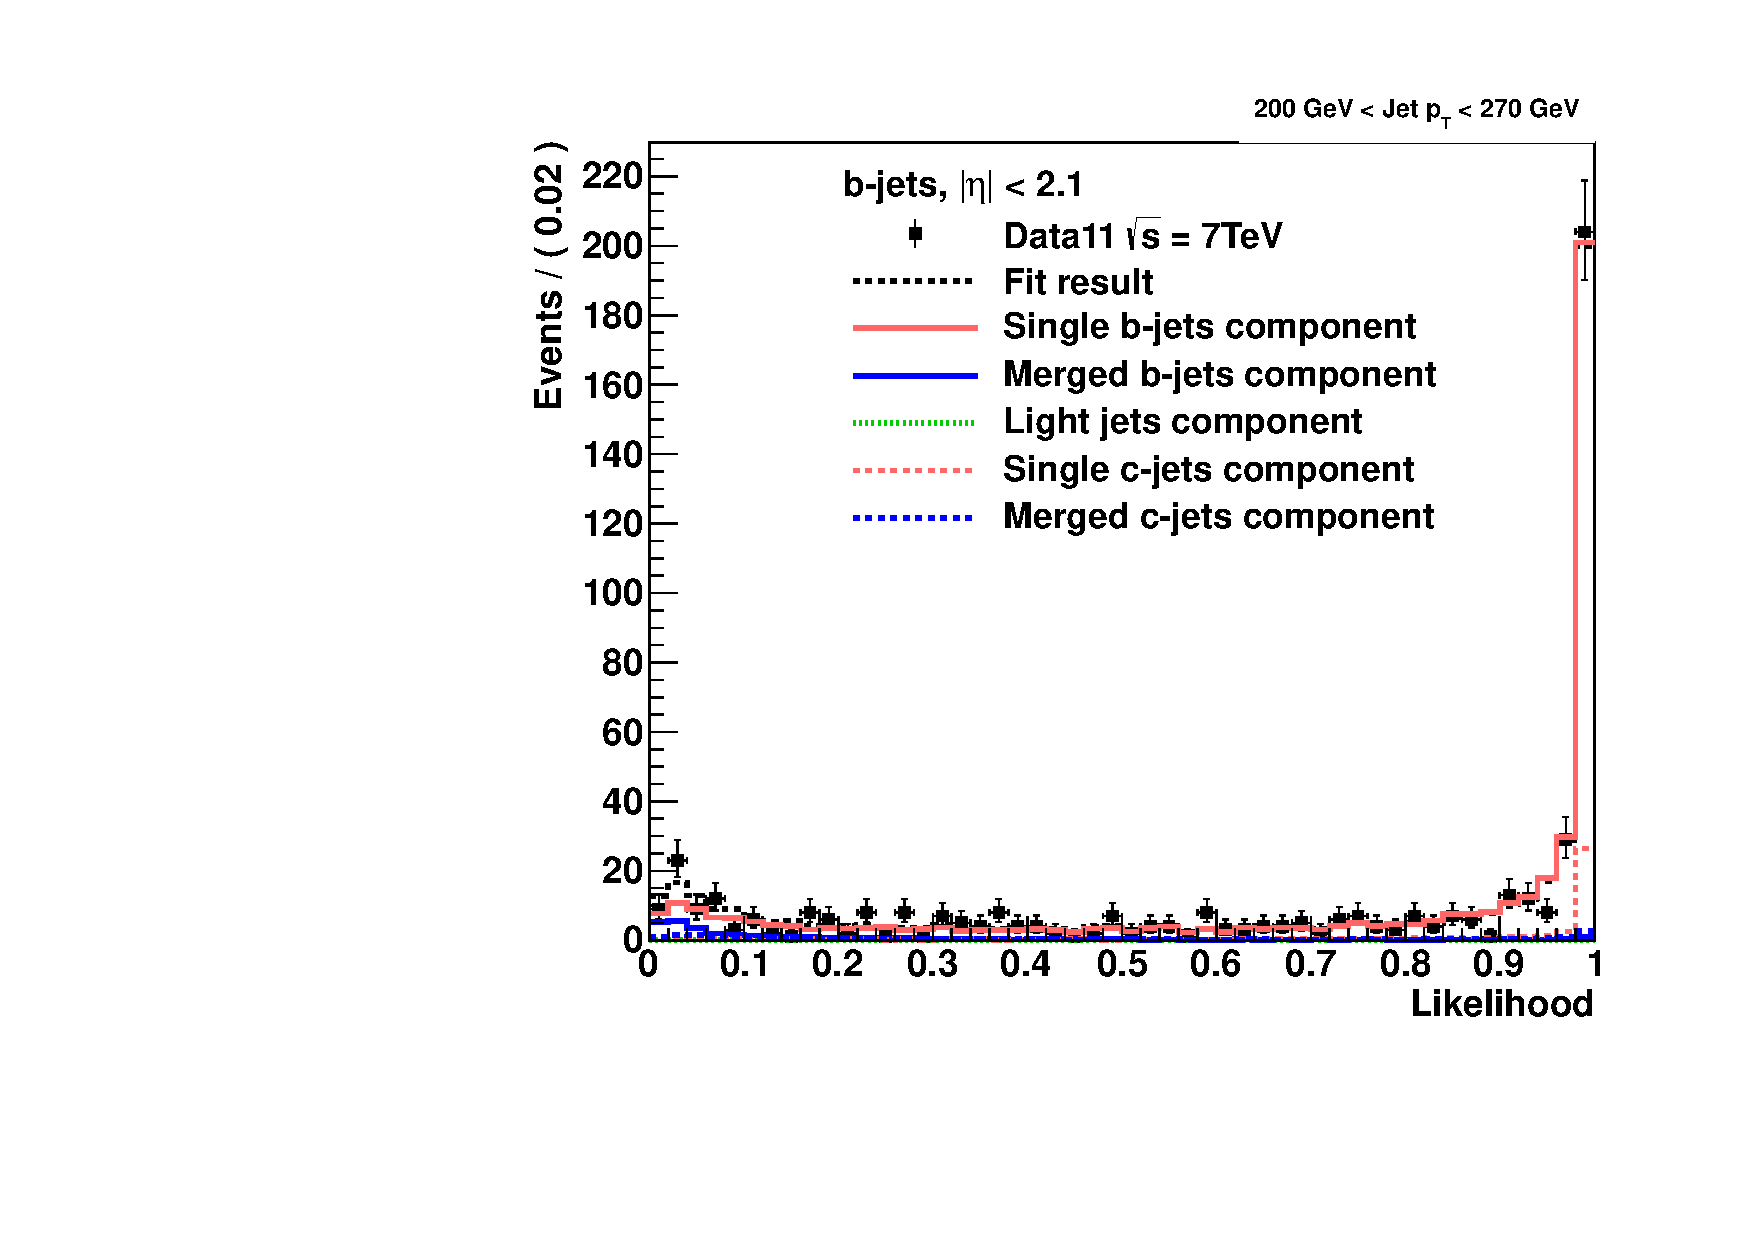
\includegraphics[width=0.7\textwidth]{FIGS/Fits/LikelihoodFit_3param_ETAFull_DataEnriched2btag_Bin5.pdf}
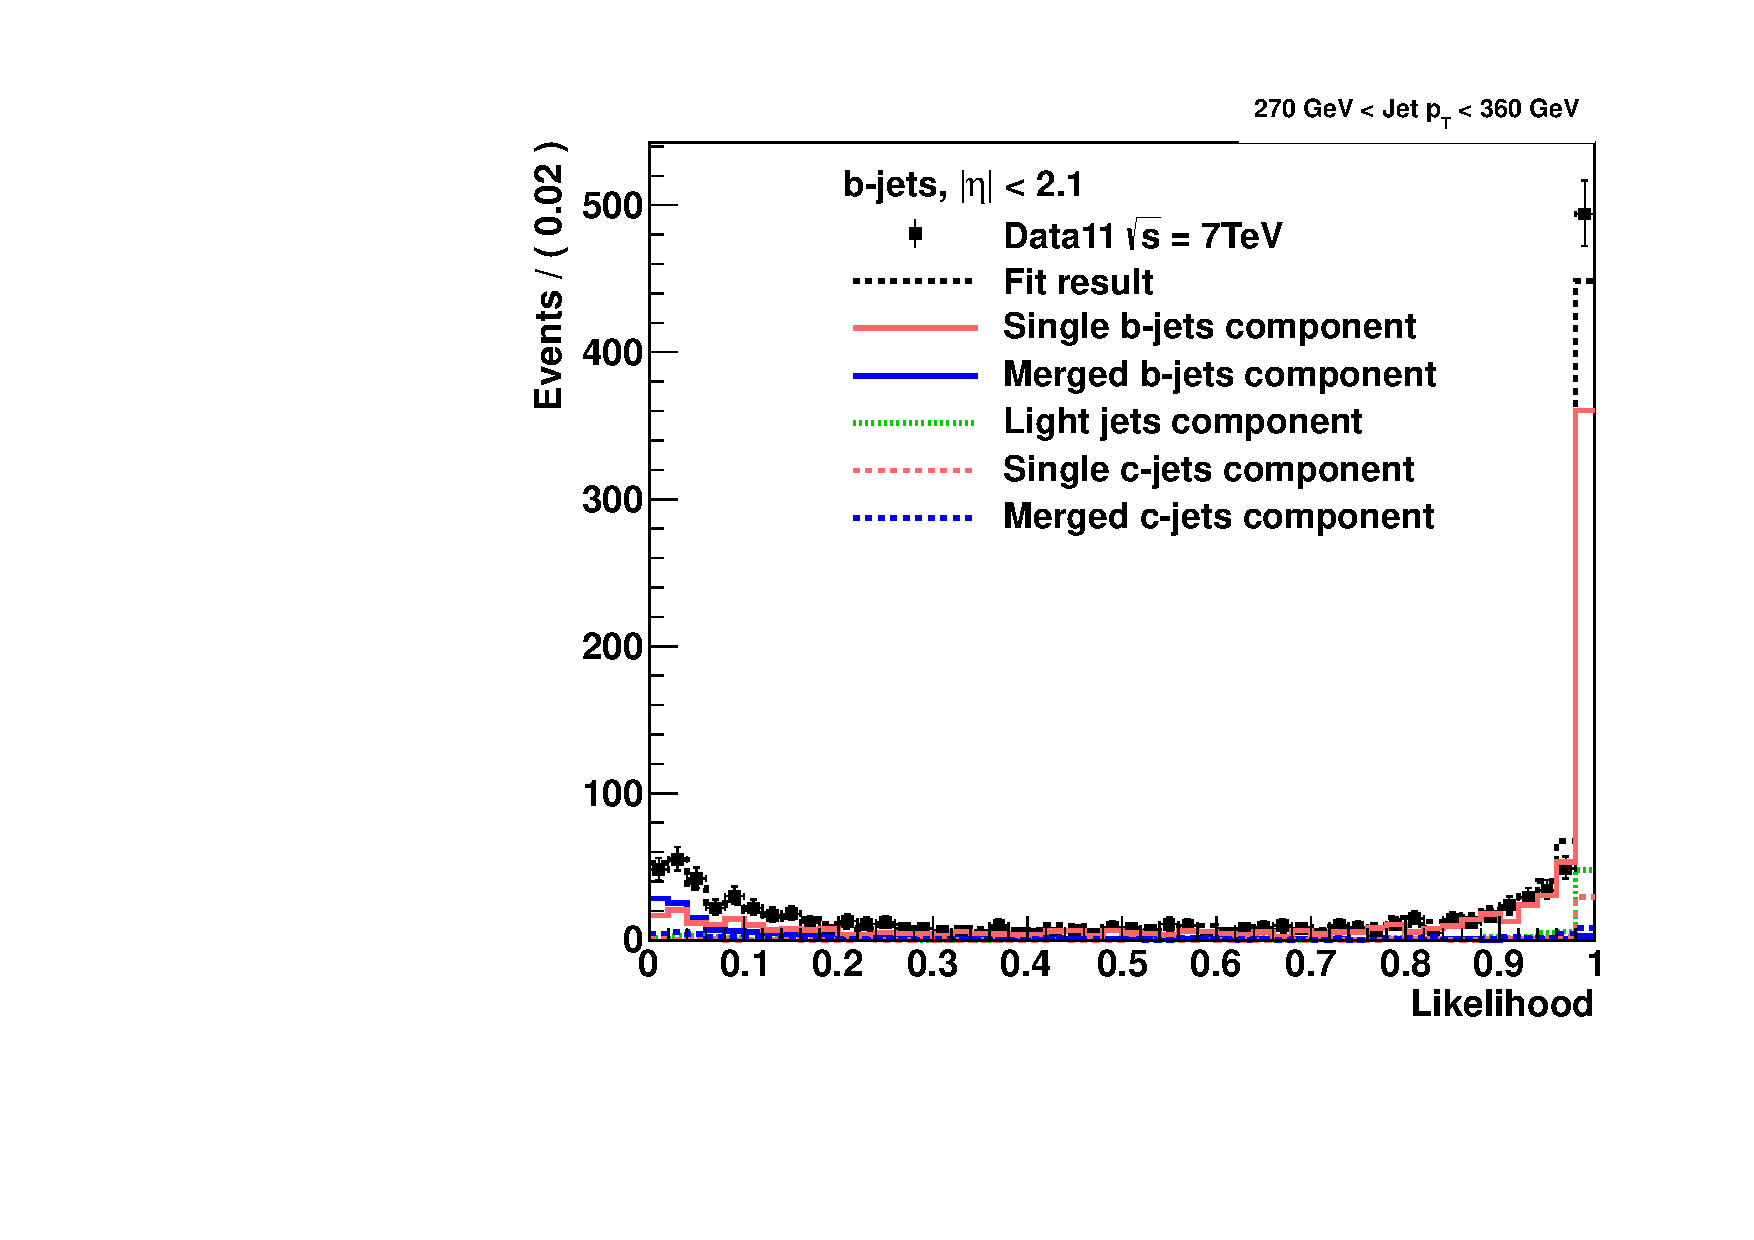
\includegraphics[width=0.7\textwidth]{FIGS/Fits/LikelihoodFit_3param_ETAFull_DataEnriched2btag_Bin6.pdf}
\caption{Monte Carlo templates for single, merged and light jets, fitted to data enriched in single $b$-jets, for jets between 200~GeV to 270~GeV and 270~GeV to 360~GeV.}
\label{fig:fitenriched2btag2}
\end{figure}




\begin{table}[!hbt] %[h]
\renewcommand{\arraystretch}{1.2}
\centering
\begin{tabular}{ | c || c | c | c ||}
  \hline
  Jet $\pt$ & \multicolumn{3}{c||}{single $b$-jet}\\ \cline{2-4}
    (GeV ) & ~~~~fit result~~~ & ~~~~stat.err.~~~~ & pythia prediction \\ \hline
   40 - 60 &  99\%  &  11\%  &  84\% \\  
   60 - 80 &  82\%  &  ~5\%  &  87\% \\ 
   80 - 110&  84\%  &  ~5\%  &  88\% \\ 
  110 - 150&  86\%  &  ~8\%  &  85\% \\ 
  150 - 200&  89\%  &  ~9\%  &  83\% \\ 
  200 - 270&  95\%  &  15\%  &  80\% \\ 
  270 - 360&  67\%  &  11\%  &  81\% \\ 
  360 - 480&  73\%  &  16\%  &  73\% \\ \hline
\end{tabular}
\caption{Measured fractions of single $b$-jets in experimental data from 2011 run, enriched in single $b$-jets.}
\label{tb:fitfractions2btagS}
\end{table}

\begin{table}[!hbt] %[h]
\renewcommand{\arraystretch}{1.2}
\centering
\begin{tabular}{ | c || c | c | c ||}
  \hline
  Jet $\pt$ & \multicolumn{3}{c||}{merged $b$-jet}\\ \cline{2-4}
    (GeV ) & ~~~~fit result~~~ & ~~~~stat.err.~~~~ & pythia prediction \\ \hline
   40 - 60 &  -1\%  &  1\%  &  1\% \\  
   60 - 80 &  -3\%  &  1\%  &  1\% \\ 
   80 - 110&  ~2\%  &  1\%  &  1\% \\ 
  110 - 150&  ~4\%  &  2\%  &  3\% \\ 
  150 - 200&  ~4\%  &  2\%  &  3\% \\ 
  200 - 270&  ~7\%  &  2\%  &  5\% \\ 
  270 - 360&  12\%  &  2\%  &  6\% \\ 
  360 - 480&  10\%  &  1\%  &  8\% \\ \hline
\end{tabular}
\caption{Measured fractions of merged $b$-jets in experimental data from 2011 run, enriched in single $b$-jets.}
\label{tb:fitfractions2btagM}
\end{table}

\begin{table}[!hbt] %[h]
\renewcommand{\arraystretch}{1.2}
\centering
\begin{tabular}{ | c || c | c | c ||}
  \hline
  Jet $\pt$ & \multicolumn{3}{c||}{light $b$-jet}\\ \cline{2-4}
    (GeV ) & ~~~~fit result~~~ & ~~~~stat.err.~~~~ & pythia prediction \\ \hline
   40 - 60 &  ~-7\%  &  11\%  &  5\% \\  
   60 - 80 &  ~17\%  &  ~6\%  &  2\% \\ 
   80 - 110&  ~~4\%  &  ~6\%  &  1\% \\ 
  110 - 150&  ~-1\%  &  ~9\%  &  1\% \\ 
  150 - 200&  ~-6\%  &  10\%  &  2\% \\ 
  200 - 270&  -17\%  &  17\%  &  3\% \\ 
  270 - 360&  ~~9\%  &  11\%  &  4\% \\ 
  360 - 480&  ~~4\%  &  16\%  &  8\% \\ \hline
\end{tabular}
\caption{Measured fractions of light $b$-jets in experimental data from 2011 run, enriched in single $b$-jets.}
\label{tb:fitfractions2btagL}
\end{table}
